% Suggested replacement of \subsection{Comparison of Wind Turbine Control Designs}
% (label subsec:ComparisonWindTurbineControlDesigns) in 04_WindTurbineControl_02_notBold.tex,
% i.e. of that subsection up to the end of the chapter file. It keeps the labels
% subsec:ComparisonWindTurbineControlDesigns, fig:EvalCrit1 and fig:CtrlCompAll, so it is meant
% to be \input instead of the existing subsection, not in addition to it.
% Figures: figures/figures_WESC25/afig01_IPCMPCbar.eps and afig01_IPCMPCpareto.eps, created with
% runParetoVerif2.m and plotParetoVerif2.m of the qLMPC repository (table figDirPareto/ParetoVerif2.mat).
% Changes to the existing text:
% - 18 m/s (second verification set, NTM class B) instead of 16 m/s
% - qLMPC on Mdl2 (no model mismatch) and on FAST (filter designs, also combined with IPC)
% - bar plot first, grouped by controller at 8 deg/s; Pareto plot in three panels
% - DELs with Woehler exponents 10 (blades, sum of the three blades) and 4 (tower), evaluated from 66 s
% TODO: reference to the section describing the qLMPC designs on FAST (notch filters, smooth
% pitch reference, controller sample time) once it is part of the chapter.

\subsection{Comparison of Wind Turbine Control Designs}
\label{subsec:ComparisonWindTurbineControlDesigns}

In a first comparison, the qLMPC was evaluated on the simplified turbine model that is also
used as its prediction model, for turbulent wind with a mean of 16\,m/s. Without any model
mismatch, it achieved large improvements over the PI baseline: the tower DEL was reduced by 23\%, 30\%, and 54\% for the pitch rate limits of
4\textdegree/s, 8\textdegree/s, and 13\textdegree/s, the blade DEL, estimated from the blade
movement, by 8\%, 13\%, and 24\%, and the power standard deviation $C_{\delta P}$ dropped to
approximately 0.22. These improvements did not hold up. Applied to the FAST model of the NREL 5-MW
turbine, the original qLMPC design increased the power tracking error instead of reducing it,
mainly due to the mismatch between the prediction model and the high-fidelity turbine, e.g.\
the structural modes not contained in the prediction model. When filters were used, the
improvements were partly recovered. With a prediction model extended by the tower fore-aft and
blade flap dynamics, notch filters at the 3P frequency and the drivetrain mode in the measured
speeds, and, for the smooth design, a longer controller sample time with a ramped pitch
reference, the qLMPC reduces the power variance on FAST again, but at the cost of the tower
loads. On the simplified model, the
rotor-effective wind filters shown in Table~\ref{tab:stddev_unified} have a similar effect: they
remove a large part of the excitation, so both the pitch activity and the improvement of the
qLMPC become smaller.

All designs are therefore compared again for the same wind, the turbulent 18\,m/s wind of the
second verification set (IEC turbulence class~B), with the pitch rate limits 4\textdegree/s,
8\textdegree/s, and 13\textdegree/s. The qLMPC is evaluated on the simplified model Mdl2 as the
ideal case without model mismatch, and on FAST v8.16 with the filter designs, both on their own
and combined with the individual pitch controller of Section~\ref{section:Individal Pitch PI Control}.
IPC and AALC are evaluated on OpenFAST with the optimized gains for each rate limit and the
AALC gains of Section~\ref{subsec:ResultsTEF} at 8\textdegree/s. All criteria are normalized by the
PI baseline on the same plant and with the same pitch rate limit, so values below unity
indicate an improvement. The blade and tower DELs are computed by rainflow counting with
W\"ohler exponents of 10 for the blades, summed over the three blades, and 4 for the steel
tower; all criteria are evaluated from 66\,s onwards to exclude the start-up. Mdl2 contains
neither blade loads nor a pitch moment. For the qLMPC on Mdl2, the standard deviation of the
tower top fore-aft acceleration replaces the tower DEL, no blade DEL is given, and $C_\text{Act}$
is calculated with a pitch moment estimated from the pitch angle, its derivatives, and the wind
speed. This estimate is fitted to FAST runs and reproduces the actuator power of the qLMPC on
FAST within 2\%.

\begin{figure}[htbp]
    \begin{center}
        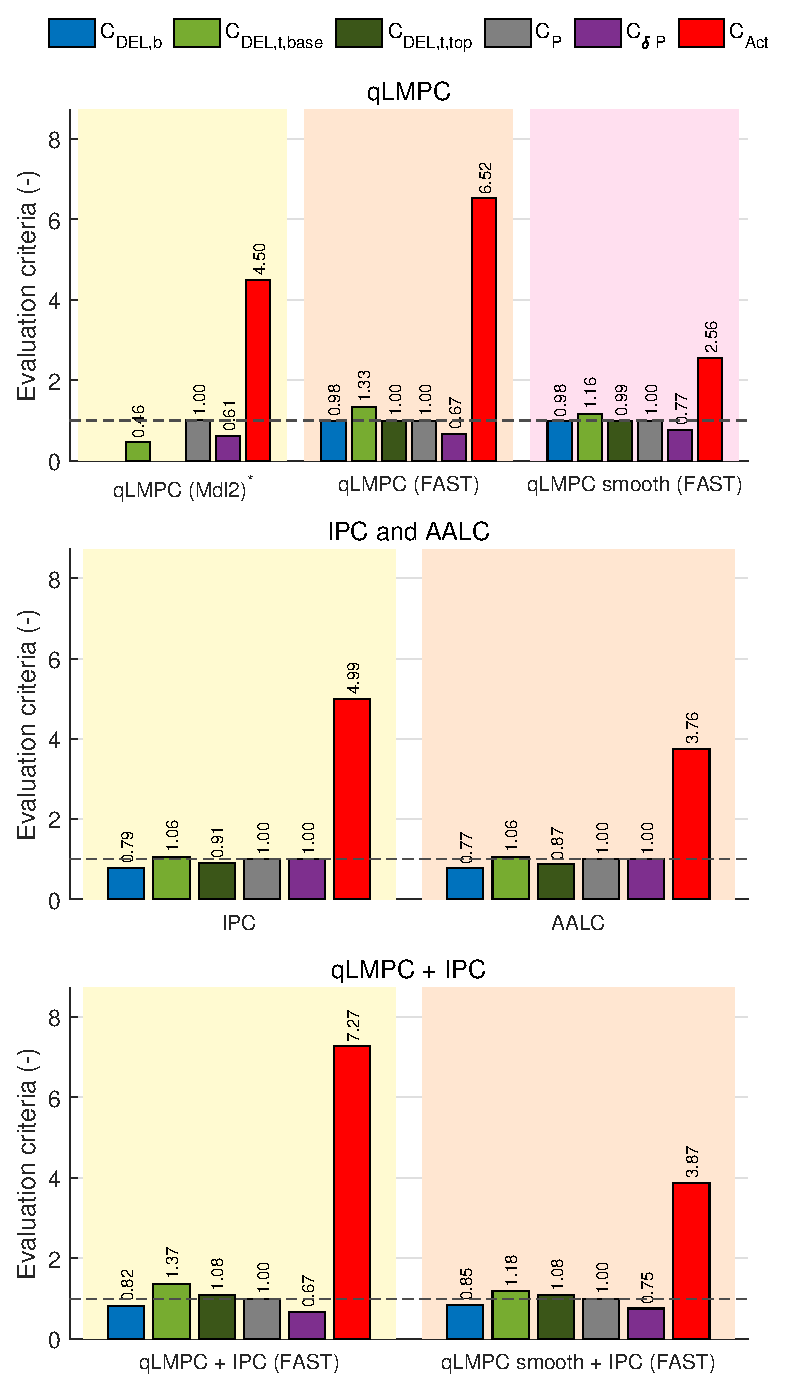
\includegraphics[width=0.55\textwidth]{figures/figures_WESC25/afig01_IPCMPCbar.eps}
        \caption[Evaluation criteria of qLMPC, IPC, and AALC for turbulent wind at a pitch rate limit of 8\textdegree/s]{Evaluation criteria of the controllers for turbulent wind (18\,m/s mean, IEC turbulence class~B, second verification set) and a pitch rate limit of 8\textdegree/s, normalized by the PI baseline with the same rate limit: blade and tower DELs $C_{\mathrm{DEL},b}$ and $C_{\mathrm{DEL},t}$, mean power $C_{\bar{P}}$, power standard deviation $C_{\delta P}$, and actuator power $C_\text{Act}$. (a)~qLMPC, (b)~IPC and AALC, (c)~qLMPC combined with IPC. $^*$qLMPC on Mdl2 (no model mismatch): $C_\text{Act}$ with the pitch moment estimated from a model fitted to FAST, $C_{\mathrm{DEL},t}$ replaced by the standard deviation of the tower top fore-aft acceleration, no blade DEL.}
        \label{fig:EvalCrit1}
    \end{center}
\end{figure}

Figure~\ref{fig:EvalCrit1} shows the evaluation criteria of all controllers at the standard
pitch rate limit of 8\textdegree/s, grouped by controller. No controller changes the mean power
$C_{\bar{P}}$; all values are within 0.5\% of the baseline.

Panel~(a) shows the qLMPC. On Mdl2, i.e.\ without model mismatch, the qLMPC reduces the power
standard deviation by 39\% and the standard deviation of the tower fore-aft acceleration by
54\%. The Verif.~2 wind is more turbulent than the test case of Section~\ref{quasiLPVMPCResults} and
falls below rated wind speed several times, so the improvements are smaller than the factors
reported there. The actuator power increases by a factor of 4.5, as the qLMPC compensates the
wind fluctuations with fast pitch action. On FAST, the qLMPC with notch filters still reduces the
power standard deviation by 33\%, but it does not reduce the blade DEL, increases the tower DEL
by 33\%, and requires the highest actuator power of all controllers without IPC, 6.5 times that
of the PI baseline. The smooth design trades part of the power smoothing, a reduction by 23\%,
for considerably less pitch activity: its actuator power of 2.6 is the lowest of all controllers,
and the tower DEL increase is halved to 16\%.

Panel~(b) shows the IPC and the AALC, which act on the blade loads. They reduce the blade DEL by
21\% and 23\%, with a small increase of the tower DEL by 6\%, and leave the power standard
deviation unchanged. The AALC achieves the larger blade load reduction at a lower actuator power
than the IPC, 3.8 compared with 5.0, as part of the load reduction is taken over by the trailing
edge flaps.

Panel~(c) shows the qLMPC designs combined with IPC. Adding IPC reduces the blade DEL by 18\%
and 15\% instead of 2\%, while the tower DEL and the power standard deviation remain close to the
values of the qLMPC alone. The additional individual pitch action increases the actuator power to
7.3 for the notch filter design and to 3.9 for the smooth design.

\begin{figure}[htbp]
    \begin{center}
        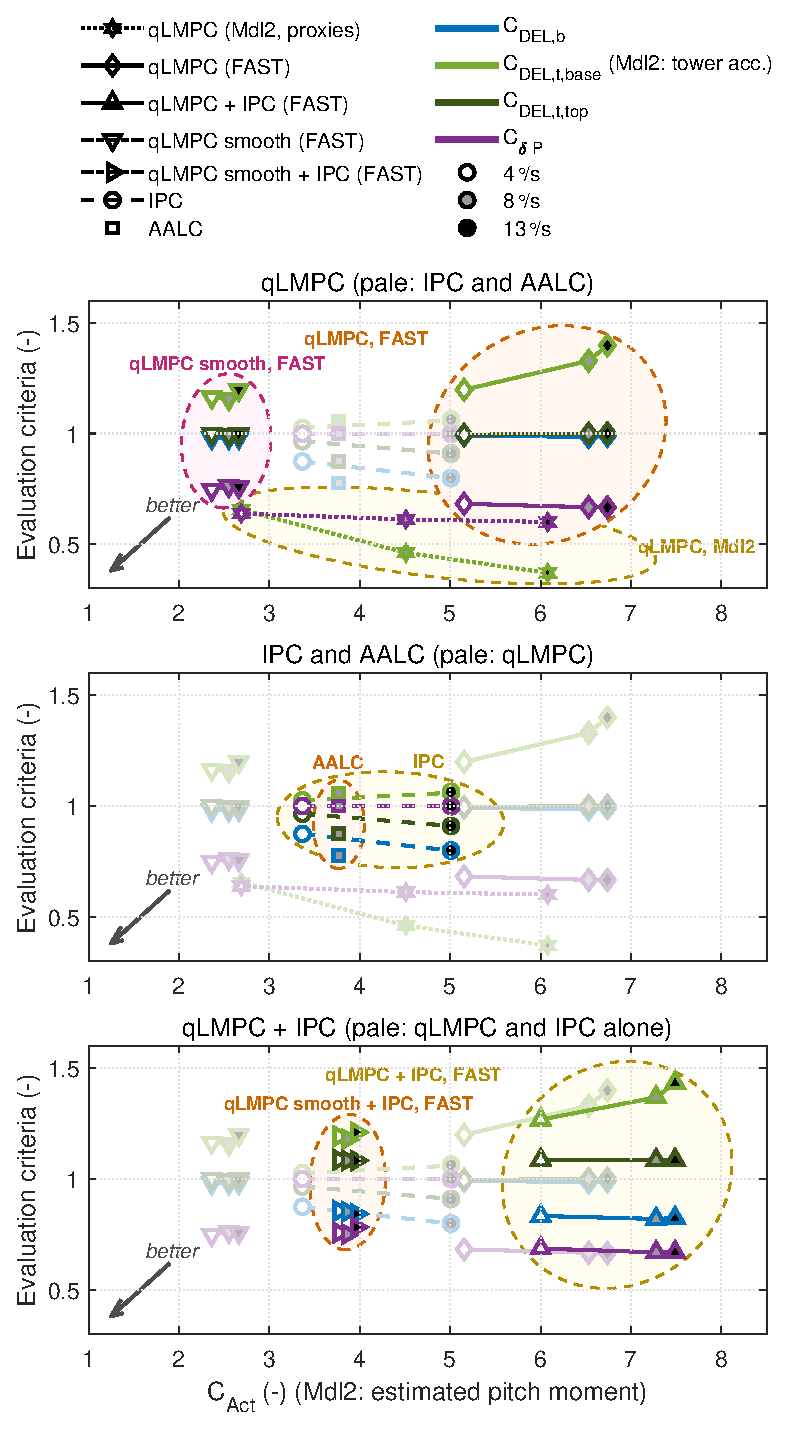
\includegraphics[width=0.55\textwidth]{figures/figures_WESC25/afig01_IPCMPCpareto.eps}
        \caption[Evaluation criteria of qLMPC, IPC, and AALC over the actuator power for turbulent wind]{Evaluation criteria $C_{\mathrm{DEL},b}$ (blue), $C_{\mathrm{DEL},t}$ (green), and $C_{\delta P}$ (purple) over the actuator power $C_\text{Act}$ for turbulent wind (18\,m/s mean, IEC turbulence class~B, second verification set), normalized by the PI baseline with the same pitch rate limit. Marker fill: pitch rate limit 4\textdegree/s (white), 8\textdegree/s (grey), and 13\textdegree/s (black). (a)~qLMPC on Mdl2 and FAST, IPC and AALC pale, (b)~IPC and AALC, qLMPC pale, (c)~qLMPC combined with IPC on FAST, qLMPC and IPC alone pale. qLMPC on Mdl2: tower top fore-aft acceleration instead of the tower DEL, $C_\text{Act}$ with the estimated pitch moment. The arrow points towards better results.}
        \label{fig:CtrlCompAll}
    \end{center}
\end{figure}

Figure~\ref{fig:CtrlCompAll} shows the blade DEL, the tower DEL, and the power standard deviation
as functions of the actuator power for all three pitch rate limits. Each line connects the
results of one controller for the rate limits of 4\textdegree/s, 8\textdegree/s, and 13\textdegree/s,
indicated by white, grey, and black marker fill. The AALC was optimized for 8\textdegree/s only and
is therefore represented by a single point per criterion. Results closer to the lower left corner
are better, as they combine lower loads or power variance with less actuator activity. Each panel
highlights one group of controllers and shows the others pale for reference.

Panel~(a) highlights the qLMPC. On Mdl2, higher pitch rate limits continuously reduce the tower
fore-aft acceleration, from 0.66 to 0.37 times the baseline, while the power standard deviation
saturates at about 0.6 and the actuator power rises from 2.7 to 6.1. On FAST, the curves of the
notch filter design lie at the highest actuator power, and higher rate limits increase the tower
DEL further, from 1.20 to 1.40, while the power standard deviation hardly improves beyond
4\textdegree/s. With a rate limit of 13\textdegree/s, this design exceeds 4\textdegree/s during 10\%
of the time, which explains the increase of the actuator power with the rate limit. The smooth
design exceeds 4\textdegree/s during only 1.3\% of the time and hence hardly depends on the rate
limit; its points form a compact cluster at the lowest actuator power. The comparison of Mdl2 and FAST shows the effect
of the model mismatch: the reduction of the power variance persists, although smaller, whereas the
tower load reduction is lost.

Panel~(b) highlights the IPC and the AALC. The IPC reduces the blade DEL from 0.87 at
4\textdegree/s to 0.79 at 8\textdegree/s; a rate limit of 13\textdegree/s brings no further benefit,
as the gains optimized for 13\textdegree/s are almost identical to those for 8\textdegree/s. The tower
DEL increases slightly with the rate limit, from 1.03 to 1.06, and the power standard deviation
remains at unity. The AALC blade DEL lies below the IPC curve, i.e.\ the AALC reaches a lower blade
DEL than the IPC with less actuator power, at the same tower DEL as the IPC at 8\textdegree/s.

Panel~(c) highlights the combination of qLMPC and IPC. Compared with the pale qLMPC curves, adding
IPC mainly shifts the blade DEL downwards and the actuator power to the right; the tower DEL and
the power standard deviation curves hardly change. The smooth design combined with IPC lies at
about the actuator power of the IPC and the AALC. It almost reaches the blade DEL reduction of the
IPC, 0.85 compared with 0.79, and in addition reduces the power standard deviation by about 24\%,
which neither IPC nor AALC achieve. Its tower DEL, however, is about 12 percentage points higher
than with IPC.

Overall, IPC and AALC remain the most effective approaches for blade load reduction, and AALC
achieves the best blade DEL at a moderate actuator power by offloading part of the pitch action
onto the trailing edge flaps. The qLMPC is the only approach that reduces the power variance, and
it keeps this property in the presence of model mismatch, with a reduction of about a third on
FAST compared with about 40\% on Mdl2. The tower load reduction that the qLMPC achieves without
model mismatch, however, is not retained on FAST, where all qLMPC designs increase the tower DEL.
The smooth qLMPC combined with IPC is the most balanced design among the qLMPC variants, as it
combines blade load reduction and power smoothing at an actuator power comparable to IPC and
AALC. The results also show that the qLMPC depends on an accurate wind speed for scheduling and
on the treatment of the high-frequency content of the measured signals, whereas IPC achieves its
load reduction without wind measurements or additional actuation hardware. These findings
highlight the trade-offs between controller complexity, sensor requirements, additional hardware
such as TEFs, and the achievable reduction of loads and power fluctuations.

The presented qLMPC exploits that individual wind turbine dynamics are well understood and can
be described in closed form as low-dimensional nonlinear ODEs. The following chapter discusses
data-driven MPC for wind farms, where wake dynamics are time- and location-dependent and cannot
be described by closed-form ODEs, yet must be accounted for in any MPC formulation.
